\documentclass[12pt, a4paper]{article}
\usepackage[T2A]{fontenc}
\usepackage{amsfonts}
\usepackage{amsmath}
\usepackage{mathabx}
\usepackage{graphicx}
\usepackage{hyperref}
\usepackage{listings}
\usepackage{color}
\usepackage{tikz}

\definecolor{dkgreen}{rgb}{0,0.6,0}
\definecolor{gray}{rgb}{0.5,0.5,0.5}
\definecolor{mauve}{rgb}{0.58,0,0.82}

\lstset{frame=tb,
  language=C++,
  aboveskip=3mm,
  belowskip=3mm,
  showstringspaces=false,
  columns=flexible,
  basicstyle={\small\ttfamily},
  numbers=none,
  numberstyle=\tiny\color{gray},
  keywordstyle=\color{blue},
  commentstyle=\color{dkgreen},
  stringstyle=\color{mauve},
  breaklines=true,
  breakatwhitespace=true,
  tabsize=2
}

\title{Основы операционных систем 1 модуль.}
\author{Андрей Тищенко}
\date{2024/2025}

\newcommand{\mytab}{\hspace{0.5cm}}

\begin{document}
    \maketitle
    \begin{center}
        \textbf{Лекция 2 сентября.}
    \end{center}
    \section{\text{Структура вычислительной системы.}}
    Вычислительная система состоит нескольких частей:
    \begin{itemize}
        \item Пользователь. (алгоритмы и алгоритмические языки)
        \item Прикладные программы. (ЦГ, matlab и т.п.)
        \item Системные программы. (системное программирование)
        \item Операционная система. (основы операционных систем)
        \item Техническое обеспечение. (архитектура ЭВМ и языки ассемблера)
    \end{itemize}
    Прекрасная притча про слепцов и слона.
    \subsection{\text{Что такое операционная система?}}
    Различные точки зрения (что такое ОС?):
    \begin{itemize}
        \item Распорядитель ресурсов.
        \item Защитник пользователей и программ.
        \item Виртуальная машина (фокусник, виртуальная память).
        \item Кот в мешке (попросил загрузить ОС, значит всё загруженное и есть ОС).
        \item Постоянно функционирующее ядро.
    \end{itemize}
    Проще сказать не что такое операционная система, а для чего она нужна и чем 
    занимается. Современные ОС это продукт эволюции вычислительных систем, поэтому 
    стоит эту эволюцию рассмотреть.
    \subsubsection{\text{Эволюция вычислительных систем}}
    Удобство, стоимость и производительность --- самые главные факторы отбора в 
    эволюции операционных система.\\
    Условные этапы развития вычислительных систем:
    \begin{enumerate}
        \item[\text{1-й период.}] (1945--1955гг.) Научно-исследовательнская работа в области вычислительной техники.
        \begin{itemize}
            \item Ламповые машины.
            \item Нет разделения персонала.
            \item Вход программы коммутацией или перфокартами.
            \item Одновременное выполнение толко одной операции.
            \item Появление прообразов первых компиляторов.
            \item Нет операционных систем.
        \end{itemize}
        \item[\text{2-й период.}] (1955-начало 60-х гг.) Начало использования вычислительных машин в научных и коммерческих целях.
        \begin{itemize}
            \item Транзисторные машины
            \item Происходит разделение персонала (появление малочисленной касты программистов)
            \item Бурное развитие алгоритмических языков (напиши $10\,000$ строк на асме и отладь, это стало причиной появления первых языков программирования)
            \item Ввод заадния колодой перфокарт
            \item Вывод результатов на печать
            \item Пакеты заданий и системы пакетной обработки.
        \end{itemize}
        \item[\text{3-й период.}] (начало 60-х годов--1980 гг.)
        Конец этого периода указан точно. Тактовая частота значительно повысилась из-за появления микросхем.
        \begin{itemize}
            \item Машины на интегральных схемах.
            \item Использование спулинга spooling. (появление процессоров ввода/вывода, которые включаются вместо центрального процессора)
            \item Планирование заданий (из-за появления магнитных дисков вместо ленты).
            \item Мультипрограммные пакетные системы. (в память загружается несколько программ, пока происходит ввод/вывод на в одной программе ЦП передаётся другой программе)
            \item Системы разделения времени (time-sharing).
            \item Интерактивная отладка программ.
            \item Виртуальная память.
            \item Появление семейств ЭВМ.
        \end{itemize}
        \mytabМультипрограммирование и эволюция вычислительных систем.
        \[\begin{tabular}{c|c}
            \textbf{Software} & \textbf{Hardware}\\
            \hline
            \text{Планирование заданий} & \text{Защита памяти}\\
            Управление памятью & Сохранение контекста\\
            Сохранение контекста & Механизм прерывания\\
            Планирование использования процессора & Привилегированные команды\\
            Системные вызовы & \\
            Средства коммуникации & \\
            Средства синхронизации &
        \end{tabular}\]
        \mytabИнтерактивная отладка стала возможна благодаря изобретению терминала, но возникла новая проблема:
        нужно хранить информацию разных пользователей так, чтобы они не могли портить данные других пользователей, 
        также потребовался единый стандарт хранения данных в компьютере.\par
        \hspace{0.5cm}Хотелось разрешить как можно большему числу пользователей одновременно пользоваться вычислительной 
        машиной. Для этого нужно было экономить оперативную память. С целью решения этой проблемы программы 
        подгружаются в машину по частям (только нужные в данный момент куски). На этой концепции основана 
        виртуальная память.\par
        \mytabСемейства ЭВМ были нужны для того, чтобы маленькие кампании могли покупать маломощные компьютеры, 
        писать свой код на них, по мере роста кампании покупать более мощные машины того же семейства и исполнять 
        такой же код без переписывания и перекомпиляции.
        \item[\text{4-й период}] (1980--2005 гг.)
        \begin{itemize}
            \item Машины на больших интегральных схемах (БИС).
            \item Персональные ЭВМ.
            \item Дружественное программное обеспечение.
            \item Сетевые и распределённые операционные системы.
        \end{itemize}
        \mytabПоскольку теперь любой человек мог стать владельцем персонального ЭВМ, 
        было необходимо создать дружелюбный интерфейс для предоставления человеку без 
        специального образования пользоваться персональной машиной.\par
        \mytabИз-за увелечения количества компьютеров увеличилась важность компьютерных 
        сетей. Пользователи, работающие на сетевой ОС должны были понимать как доставать 
        и обрабатывать файлы из сервера.\par
        \mytabВладелец распределённой операционной системы не 
        должен понимать, где находится его файл, обращение к файлу на локальной машине 
        и к файлу на сервере, управляемом распределённой ОС, должно выглядеть для пользователя 
        одинаково.\par
        \mytabШирокое использование ЭВМ в быту, образовании и на производстве.
        \item[\text{5-й период}] (2005-?? гг.)
        \begin{itemize}
            \item Машины на многоядерных процессорах.
            \item Мобильные компьютеры.
            \item Высокопроизводительные вычислительные системы.
            \item Облачные технологии.
            \item Виртуализация выполнения программ.
        \end{itemize}
        \mytabМожно виртуализовать программы и операционные системы.\par
        \mytabПериод Глобальной компьютеризации.
    \end{enumerate}
    \subsection{Основные функции ОС}
    \begin{itemize}
        \item Планирование заданий и использования процессора. (кто и после кого будет выполняться)
        \item Обеспечение программ средствами коммуникации и синхронизации.
        \item Управление памятью.
        \item Управление файловой системой.
        \item Управление вводом-выводом.
        \item Обеспечение безопасности.
    \end{itemize}
    Операционные системы существуют потому что на данный момент их существование 
    --- это разумный способ использования вычислительных систем.
    \section{Архитектурные особенности построения ОС}
    \subsection*{Внутреннее строение ОС (разновидности)}
    \begin{center}
        Монолитное ядро.
    \end{center}
    \begin{itemize}
        \item Каждая процедура (функция) может вызвать каждую.
        \item Все процедуры работают в привилегированном режиме.
        \item Ядро совпадает со всей операционной системой.
        \item Пользовательские программы взаимодействуют с ядром через системные вызовы.
    \end{itemize}
    \begin{center}
        Многоуровневые (Layered) системы.
    \end{center}
    \begin{itemize}
        \item Процедура уровня $K$ может вызывать только процедуры уровня $K-1$
        \item Все или почти все уровни работают в привилегированном режиме
        \item Ядро совпадает или почти совпадает со всей операционной системой
        \item Пользовательские программы взаимодействуют с ОС через интерфейс пользователя
    \end{itemize}
    \mytabСамый низкий уровень --- Hardware. Самый высокий --- интерфейс пользователя.
    В самой первой такой машине выглядело так:
    \begin{enumerate}
        \item Интерфейс пользователя.
        \item Управление ввода вывода.
        \item Связь с консолью.
        \item Управление памятью.
        \item Планирование заданий и программ.
    \end{enumerate}
    \mytabРаботает медленнее, чем система монолитного ядра, но отладка и модификация сильно упрощается.
    \begin{center}
        Микроядерная (microkernel) архитектура.
    \end{center}
    Функции микроядра:
    \begin{itemize}
        \item Взаимодействие между программами.
        \item Планирование использования процессора.
        \item Первичная обработка прерываний и процессов ввода вывода
        \item Управление памятью.
    \end{itemize}
    Устройство системы:
    \begin{itemize}
        \item Микроядро составляет лишь малую часть ОС.
        \item В привилегированном режиме работает только микроядро.
        \item Взаимодействие частей ОС между собой и с программами пользователей путем передачи сообщений через микроядро.
    \end{itemize}
    \mytabВсе части ОС, кроме микроядра, могут быть заменены без прерывания работы ОС. Микроядро сразу же сможет обратиться 
    к заменённой части системы.\par
    \mytabМикроядро в таком концепте работает весьма медленно, поэтому на практике для повышения быстродействия функционал микроядра расширили.
    \begin{center}
        Виртуальные машины
    \end{center}
    Каждому пользователю предоставляется своя копия виртуального hardware
    \begin{center}
        Новая микроядерная архитектура (экзоядерная архитектура).
    \end{center}
    \begin{itemize}
        \item Взаимодествие между программами 
        \item Выделение и выспобождение физических ресурсов 
        \item Контроль прав доступа
    \end{itemize} 
    \mytabВся остальная функциональность выделяется на поддержание абстракций, которые разделены на библиотеки. 
    Считается спорным подходом и на практике не используется (только в учебных ОС).
    \begin{center}
        Смешанные системы.
    \end{center} 
    Монолитное ядро - необходимость перекомпиляции при каждом изменении, сложность отладки, высокая скорость работы.\\
    Многоуровневые системы - необходимость перекомпиляции при изменениях, отлаживается только изменённый уровень, меньшая скорость работы.\\
    Микроядро - простота отладки, возможность замены компонент, без перекомпиляции и остановки системы, очень медленные.\\
    Все три подхода используются в совеременных ОС.
    \section{Понятие процесса. Операции над процессами.}
    \begin{center}
        Уточнение терминологии
    \end{center}
    Термин \textit{программа} - не может использоваться для описания происходящего внутри ОС.\\
    Термин \textit{задание} - не может использоваться для описания происходящего внутри ОС.\\
    Изначально эти термины были придуманы для статических объектов, а нам нужно описывать динамические 
    объекты.\\
    Введём термин \textit{процесс} для описания динамических объектов.\\
    Теперь под \textit{процессом} будем понимать совокупность:
    \begin{itemize}
        \item набора исполняющихся команд
        \item ассоциированных с ним ресурсов 
        \item текущего момента его выполнения
    \end{itemize} 
    \mytab Вся эта совокупность находится под управлением операционной системы.\par
    \textbf{Важно:} Процесс $\neq$ программа, которая исполняется.
    \begin{itemize}
        \item для исполнения одной программы может организовываться несколько процессов 
        \item В рамках одного процесса может исполняться несколько программ 
        \item В рамках процесса может исполняться код, отсутствующий в программе.
    \end{itemize}
    \begin{center}
        Состояния процесса
    \end{center}
    \begin{enumerate}
        \item Исполняется 
        \item Не исполняется
    \end{enumerate}
    Новые процессы не исполняются. Переход из состояний происходит в случае 
    выбора его для исполнения или приостановки. После исполнения процесс выходит из ОС.\par
    Примитивная система, которая не является верной, так как процесс может "не исполняться разными способами".
    \begin{enumerate}
        \item Готовность
        \item Исполнение
        \item Ожидание
    \end{enumerate}
    Новые процессы попадают в состояние готовности. Выбор готового процесса для исполнения прерывает в состояние исполнения. 
    В случае прерывания исполняемого процесса он переходит в состояние готовности. Если для исполнения нужно дождаться 
    какого-то события, то он переходит в состояние ожидания, после исполнения ожидаемого, он переходит в состояние готовности.\\
    Однако эту схему тоже стоит дополнить:
    \begin{enumerate}
        \item Рождение
        \item Готовность
        \item Исполнение 
        \item Ожидание
        \item Закончил исполнение
    \end{enumerate}
    Новые процессы попадают в состояние рождения, после прохождения допуска к планированию процесс попадает в состояние готовности.
    При завершении работы процесса он попадает в состояние "закончил исполнение".\\
    \textbf{Важно:} переход между состояниями процесса осуществляет ОС.

    \begin{center}
        Лекция 16 сентября
    \end{center}
    \underline{\textit{Операции над процессами:}}
    \begin{itemize}
        \item Создание процесса - завершение процесса
        \item Запуск процесса - приостановка процесса
        \item блокировка процесса - разблокирование процессса 
        \item изменение приоритета
    \end{itemize}
    Чтобы ОС могла взаимодействовать с процессами, она должна иметь какое-то представление об этом объекте. Эта информация хранится в PCB (process control block).\\
    \underline{\textit{Содержимое PCB}}
    \begin{itemize}
        \item Состояние процесса
        \item Програмнный счётчик (следующая команда в процессе)
        \item содержимое регистров
        \item данные для планирования использования процессора и управления памятью
        \item учётная информация
        \item сведения об устройствах ввода-вывода, связанных с процессом (возможно файлы, с которыми взаимодействует).
    \end{itemize}
    Регистровый контекст: программный счётчик, содержимое регистров.\\
    Всё остальное входит в системный контекст.\\
    Всё, что лежит в PCB лежит в ядре ОС, код и данные программы называются пользовательским контекстом, входят в адресное пространство процесса.\\
    \underline{\textit{Создание процесса:}}
    \begin{itemize}
        \item Присвоение идентификационного номера
        \item Порождение нового PCB с состоянием процесса "рождение"
        \item Выделение ресурсов (из ресурсов родителя и ОС)
        \item Занесение в адресное пространство кода и установка значения программного счётчика. Может создаться дубликат родителя, владеющий всей информацией родителя до момента желания создать дочерний процесс. Информация процесса может быть получена из файла (пользовательский контекст убирается, вместо него через системный вызов открывается исполняемый файл и подгружается как пользовательский контекст).
        \item Окончание заполнения PCB
        \item Изменение состояния процесса на "готовность"
    \end{itemize}
    \underline{\textit{Завершение процесса:}}
    Это состояние необходимо для того, чтобы родитель мог узнать, по какой причине ребёнок завершил процесс.
    \begin{itemize}
        \item Изменение состояния процесса на "закончил исполнение"
        \item Освобождение ресурсов (остаётся только PCB процесса, в нём остаётся учётная информация, родитель)
        \item Очистка соответствующих элементов в PCB
        \item Сохранение в PCB информации о причинах завершения.
    \end{itemize}
    После окончания родительского процесса некоторые ОС убивают всех его детей, а некоторые (например Windows и Unix) позволяют детям жить.\\
    Но в таком случае возникает вопрос с новым родителем. Например у процесса 251 был ребёнок 1000, после окончания 251 1000 продолжил работать, ОС создала новый процесс 251, который не должен являться родителем 1000. Поэтому осиротевшие процесса усыновляются процессами, которые существуют, пока ОС не прекратит работу.\\
    Если процессы используют какой-то ресурс (например файл), ему присваивается счётчик, равный количеству процессов, использующих этот ресурс. Освобождение происходит если один из процессов явно это попросил или если счётчик стал равен нулю.\\
    \underline{\textit{Запуск процесса:}}
    \begin{itemize}
        \item Изменение состояния процесса на "исполнение"
        \item Обеспечение наличия в оперативной памяти информации, необходимой для его выполнения
        \item Восстановление значений регистров
        \item передача управления по адресу, на который указывает программный счётчик.
    \end{itemize}
    PCB меняется только при переключении состояния процесса. Во время работы процесса ничего в PCB не заносится (так как это было бы непроизводительно).
    \underline {\textit{Приостановка процесса:}}
    \begin{itemize}
        \item Автоматическое сохранение программного счётчик и части регистров (работа hardware)
        \item Передача управления по специальному адресу (hardware)
        \item Сохранение динамической части... UNFINISHED
    \end{itemize}
    \underline{\textit{Блокирование процесса}}
    \begin{itemize}
        \item Сохранение контекста процесса в PCB.
        \item Обработка системного вызова (разбираемся, чего мы ждём)
        \item Перевод процесса в состояние "ожидание"
    \end{itemize}
    \underline{\textit{Разблокирование процесса:}}
    \begin{itemize}
        \item Уточнение тоо, какое именно событие произошло
        \item Проверка наличия процесса, ожидающего этого события
        \item Перевод ожидающего процесса в состояние "готовность"
        \item Обработка произошедшего события
    \end{itemize}
    \section{Кооперация процессов и основные аспекты ее логической организации}
    \underline{\textit{Основные причины объединения усилий:}}
    \begin{itemize}
        \item Повешение скорости решения задач.
        \item Совместное использование данных.
        \item Модульная конструкция какой-либо системы.
        \item Для удобства работы пользователя (например, отладчик).
    \end{itemize}
    \textit{Кооперативные или взаимодейтсвующие процессы} - это процессы, которые влияют на поведение друг друга путем обмена информацией.\\
    \underline{\textit{Категории средств взаимодействия:}}
    \begin{itemize}
        \item Сигнальные (переданная информация зачастую ограничивается битами).
        \item Канальные (создание логического канала связи. Данные из одного процесса могут быть получены при желании другого, тогда произойдёт передача запрошенных данных)
        \item Разделяемая память (доступна обоим процессам).
    \end{itemize}
    \underline{\textit{Как устанавливаестя связь}}
    \begin{itemize}
        \item Нужна или не нужна инициализация?
        \item Способы адресации
        \begin{enumerate}
            \item Прямая адресация
            \begin{itemize}
                \item симметричная
                \item асимметричная
            \end{itemize}
            \item Непрямая или косвенная адресация
        \end{enumerate}
    \end{itemize}
    \underline{\textit{Информационная валентность процессов и средств связи}}
    \begin{itemize}
        \item Сколько процессов может быть ассоциировано с конкретным средством связи?
        \item Сколько идентичных средств связи может быть задействовано между двумя процессами?
        \item Направленность связи
        \begin{itemize}
            \item Симплексная связь (только в одну сторону)
            \item Полудуплексная связь (двусторонняя, но только по очереди, как рация)
            \item Дуплексная связь (двусторонняя)
        \end{itemize}
    \end{itemize}
    \begin{center}
        Лекция 23 сентября.
    \end{center}
    \section*{Основные аспекты логической организации передачи информации}
    \subsection*{Особенности канальных средств связи}
    \underline{\textit{Буферизация}}
    \begin{itemize}
        \item Буфера нет (нулевая ёмкость). Процесс-передатчик всегда обязан ждать приёма
        \item Буфер конечной ёмкости. Процесс-передатчик обязан ждать освобождения места в буфере перед продолжением работы.
        \item Буфер неограниченной ёмкости (нереализуемо!). Процесс-передатчик никогда не ждёт.
    \end{itemize}
    \underline{\textit{Модели передачи данных}}
    \begin{itemize}
        \item Потоковая модель. Операции приёма/передачи не интересуются содержимым данных и их происхождением. Данные не структурируются.
        \item Модель сообщений. На передаваемые данные накладывается определённая структура.
    \end{itemize}
    \underline{\textit{Потоковая модель - pipe}}\par
    Источники вкладывают информацию порциями любого размера и\\
    могут считывать эти порции в любом размере. Через pipe могут общаться\\
    только процессы, имеющие общего предка, создавшего pipe. Это происходит\\
    потому что о положении начала и конца pipe знает только его создатель\\
    (и дети). Без средств синхронизации это сторого односторонняя связь.\\
    \underline{\textit{Потоквая модель - FIFO}}\par
    Представляет собой pipe c помеченным входом и выходом, что позволяет\\
    неродственным процессам общаться через него.\\
    \underline{\textit{Модель сообщений}}\par
    Сообщения в pipe имеют чёткие границы, прочитать сообщение можно\\
    только целиком. У принимающего процесса пропадает возможность\\ 
    получать данные в произвольном размере.
    \subsection*{Надёжность средств связи}
    \begin{center}
        Средство связи считается надёжным, если:
    \end{center}
    \begin{itemize}
        \item Нет потери информации
        \item Нет повреждения информации
        \item Нет нарушения порядка поступления информации
        \item Не появляется лишняя информация
    \end{itemize}
    Современные машины считаются надёжными.
    \subsection*{Как завершается связь}
    \begin{itemize}
        \item Нужны ли специальные действия для прекращения использования средства связи?
        \item Как влияет прекращение использования средства связи одним процессом на поведение других участников взаимодействия?
    \end{itemize}
    \section*{Нити исполнения (threads)}
    Для реализации многопоточности нужно из основного процесса создать ещё один процесс. Переключить контекст, запросить доступ к общей памяти (или другому средству связи). Такие накладные расходы
    нужны для реализации простейшей многопоточности. На практике из-за накладных расходов это работате ещё медленнее. Поэтому придумали thread'ы.\\
    На удивление хорошо поведение процесса можно сравнить с игрушечной железной дорогой. Шпалы принимаются за инструкции, развилки --- условные переходы. Станции --- данные со стека или input/output.\\
    Сам поезд можно принимать за регистры и данные в стеке.\\
    Если поставить две такие дороги рядом, то можно получить аналог второго процесса.\\
    А если поставить на те же рельсы второй поезд, можно получить аналог thread. Так как поезда разные, у них разные данные на регистрах и в стеке, всё остальное у них общее, так же должна присутствовать информация, позволяющая различать поезда между собой.\\
    \underline{Процесс}: системный контекст, регистровый контекст, код, данные вне стека, стек.\\
    \underline{Нить исполнения}: системный контекст нити, регистровый контекст, стек.\\
    При появлении процесса нить всего одна (называется главной нитью или master нитью). Нити также могут находиться в состоянии готовности, ожидания, исполнения и т.д.\\
    Нить находится в состоянии
    \begin{itemize}
        \item Готовности, если нет ни одной нити в состоянии исполнения и есть хотя бы одна в состоянии готовности
        \item Ожидания, если нет ни одной нити в состоянии готовности и исполнениия.
        \item Исполнения, если хотя бы одна из нитей находится в состоянии исполнения.
        \item Закончил исполнения, если все его нити находятся в состоянии закончил исполнение.
    \end{itemize}
    По-прежнему нужно тратить ресурсы на создание новой нити
    (нить создаётся легче, чем процесс). Между нитями нет
    нужды создавать дополнительные средства связи, так как
    внестековое пространство у них и так общее. Переключение
    контекста между нитями происходит быстрее, чем между
    процессами. Везде выиграли.
    \section*{Алгоритмы синхронизации}
    \subsection*{Активности и атомарные операции}
    \textit{Активность} --- последовательное выполнение ряда действий, направленных на достижение определённой цели.\\
    Активность: приготовление бутерброда.
    \begin{itemize}
        \item Отрезать ломтик хлеба
        \item Отрезать ломтик колбасы
        \item Намазать хлеб маслом
        \item Положить колбасу на хлеб
    \end{itemize}
    Каждый элемент активности является атомарным (неделимым). Во время операции никуда отвлекаться нельзя, между ними - можно.\\
    Пусть активность P: a b c, Q: d e f. (какие-то операции)\\
    При последовательном выполнении PQ: a b c d e f.\\
    Псевдопараллельное выполнение\\
    (режим разделения времени): a d b e c f. В таком случае атомарные операции одного процесса расположены в правильном порядке, поэтому на итоговый результат не влияет.
    \begin{center}
        Детерминированность выбора
    \end{center}
    P: $x = 2,\ y = x - 1$, Q: $x = 3,\ y = x + 1$\\
    При последовательном выполнении PQ: (x, y) = (3, 4).\\
    Однако перестановка $x = 2, x = 3, y = x - 1, y = x + 1\Rightarrow$ (x, y) = (3, 3), приводит к недетерминированности.
    \subsection*{Условия Бернстайна}
    Пусть P: $1.\ x = u + V,\ 2.\ y = x\cdot w$. Входные данные: $R_1 =\{u,\ v\}$, $R_2 = \{x,\ w\}$. Выходные данные: $W_1 = \{x\},\ W_2 = \{y\}$.\\
    Вход для активности $R(P) = \{u,\ v,\ x,\ w\}$. Выход для активности $W(P) = \{x,\ y\}$\\
    Тогда достаточные условия детерминированности Бернстайна:
    \begin{enumerate}
        \item $W(P)\cap W(Q) = \emptyset$
        \item $W(P) \cap R(Q) = \emptyset$
        \item $R(P) \cap W(Q) = \emptyset$
    \end{enumerate}
    Если все условия выполнены, то набор активностей $\{P,\ Q\}$ является детерминированным.\\
    В недетерминированных наборах всегда встречается race condition (состояние гонки).\\
    Избежать недетерминированного поведения при неважности очередности доступа можно с помощью \textit{взаимоисключения} (mutual exclusion).
    \begin{center}
        Критическая секция
    \end{center}
    Пример про трёх студентов и пиво в пятницу. Каждый из студентов приходит в комнату, видит, что пива нет и уходит в магазин покупать. В итоге каждый из них купил пива на троих и получилась славная пьянка. Поэтмоу операцию уйти за пивом, купить на всех и вернуться с пивом стоит заменить атомарной операцией. Тогда первый студент выполнит эту операцию и двум другим ничего делать не придётся.\\
    \underline{Структура кооперативного процесса}
    \begin{lstlisting}
    while (some condition) {
    entry section
        critical section
    exit section
        remainder section
    }
    \end{lstlisting}
    \begin{center}
        Требования к программным алгоритмам
    \end{center}
    \begin{enumerate}
        \item Программный алгоритм должен быть программным (проблемы решаются в коде, а не на уровне hardware)
        \item Нет предположений об относительных скоростях выполнения и числе процессоров
        \item Выполняется условие взаимоисключения (mutual exclusion) для критических участков.
        \item Выполняется условие прогресса (progress).
        \begin{itemize}
            \item Решения принимают только те, кто готов войти в критическую секцию 
            \item Решение должно приниматься за конечное время
        \end{itemize} 
        \item Выполняется условие ограниченного ожидания (bound waiting). Для каждого процесса можно сказать, какое максимальное (конечное) количество процессов он может пропустить, после чего гарантированно пройдёт в критическую секцию.
    \end{enumerate}
    \begin{center}
        \textbf{Лекция 30 сентября}
    \end{center}
    Подробнее о пункте 3. Мы хотим заставить участки процесса выполняться атомарно по отношению процессам, входящим в набор взаимодействующих процессов. Никакие два процесса из набора не могут оказаться в критическом участке в состоянии исполнения или готовности одновременно.
    \subsection*{История придумывания алгоритма синхронизации}
    \subsubsection*{Запрет прерываний}
    Существует команда Client Disable Interrupt, она говорит процессору отключить прерывания (кроме критических ошибок (nonmaskable interrupt) и прерываний, созданных пользователем). Также есть команда, возвращающая процессору возможность видеть прерывания. Если перед критической секцией поставить запрет на прерывания, а после этой секции включить прерывания, то процессы внутри будут выполняться атомарно.\\
    Минусы: бесконечный цикл внутри критической секции может быть прерван только выключением вычислительной машины. Поэтому такой метод используется только при программировании на уровне ядра.
    \subsubsection*{Переменная ``замок''}
    Оборачивать код в нечто похожее на
    \begin{lstlisting}
    shared int lock = 0;
    while (lock == 1);
    lock = 1;
    critical section
    lock = 0;
    \end{lstlisting}
    Минусы: оба процесса хотят войти в критическую секцию, первый проходит проверку на lock, заходит внутрь, но сделать lock = 1 он не успевает, так как у него забирают управление. Второй процесс входит в секцию, проверяет lock, заходит в критическую секцию, ставит lock = 1, после чего у него забирают управление. В результате мы имеем два процесса, один из которых исполняется в критической секции, а другой - в готовности в этой же критической секции.
    \subsubsection*{Строгое чередование}
    Пусть у нас два процесса. Оборачиваем критическую секцию следующим образом:\\
    \begin{lstlisting}    
    shared int turn = 1;
    \end{lstlisting}
    $Process_0$
    \begin{lstlisting}
    while (condition) {
        while (turn != 0);
            critical section
        turn = 1;
        remainder section
    }
    \end{lstlisting}
    $Process_1$
    \begin{lstlisting}
    while (condition) {
        while (turn != 1);
            critical section
        turn = 0;
        remainder section
    }
    \end{lstlisting}
    Процессы не могут одновременно находиться в критической секции, так как тогда переменная turn должна быть 0 и 1 одновременно, что невозможно.\\
    Однако условие прогресса нарушается. Пусть у $Process_0$ долгая remainder section, а у $Process_1$ обе секции короткие. Тогда первый процесс может прокрутиться внутри цикла и встать в очередь на вход в критическую секцию. Тем временем нулевой процесс всё ещё в remainder section и не может поставить флаг для первого процесса.
    \subsubsection*{Флаги готовности}
    Пусть у нас два процесса. Оборачиваем критическую секцию следующим образом:
    \begin{lstlisting}
        shared int ready[2] = {1, 0};
    \end{lstlisting}
    $Process_0$
    \begin{lstlisting}
        
    while (condition) {
        ready[0] = 1;
        while (ready[1]);
            critical section
        ready[0] = 0;
        remainder section
    }
    \end{lstlisting}
    $Process_1$
    \begin{lstlisting}
    while (condition) {
        ready[1] = 1;
        while (ready[0]);
            critical section
        ready[1] = 0;
        remainder section
    }
    \end{lstlisting}
    Здесь нарушается вторая часть условия прогресса, так как оба процесса могут одновременно быть готовыми ко входу в критическую секцию, тогда они оба будут крутить бесконечный цикл по очереди.
    \subsubsection*{Алгоритм Петерсона}
    Совмещаем флаг и переменную готовности.
    \begin{lstlisting}
    shared int ready[2] = {1, 0};
    shared int turn;
    \end{lstlisting}
    $Process_0$
    \begin{lstlisting}
    while (condition) {
        ready[0] = 1;
        turn = 1;
        while (ready[1] && turn == 1);
            critical section
        ready[0] = 0;
        remainder section
    }
    \end{lstlisting}
    $Process_1$
    \begin{lstlisting}
    while (condition) {\
    ready[1] = 1;
    turn = 0;
    while (ready[0] && turn == 0);
        critical section
    ready[1] = 0;
    remainder section
    }
    \end{lstlisting}
    В этом случае для двух процессов все условия выполняются.
    \subsubsection*{Bakery algorithm}
    Если бы алгоритм придумали в России, то назвали бы алгоритм регистратуры в поликлинике (так как пекарни на западе выпекают заказы, а не предлагают готовый ассортимент).
    \begin{center}
        Основные идеи
    \end{center}
    \begin{enumerate}
        \item Процессы можно сравнивать по именам.
        \item Перед входом в критическую секцию процессы получают талончик с номером.
        \item Первым в критическую секцию входит процесс с наименьшим номером на талоне.
        \item Выписывание талона - неатомарная операция. Могут быть талоны с одинаковыми номерами
        \item При совпадении номеров на талоне первым входит процесс с меньшим значением имени процесса.
    \end{enumerate}
    Последние два алгоритма прекрасно работали до 2005 года. В один роковой день появились многоядерные процессоры. Теперь разные ядра могли писать в одну и ту же память, в результате чего одно ядро могло записать в память одно число, после чего считать оттуда же другое, ведь с этой памятью поработало другое ядро.\\
    Для решения проблемы было принято решение ослабить консистентность памяти.
    \subsection*{Аппаратная поддержка}
    \subsubsection*{Команда Test-And-Set}
    Выполняет нечто похожее на это:
    \begin{lstlisting}
    int Test_And_Set (int* a) {
        int tmp = *a;
        *a = 1;
        return tmp;
    }
    \end{lstlisting}
    Используется для сокращение прологов и эпилогов:
    \begin{lstlisting}
    shared int lock = 0
    while (condition) {
        while(Test_And_Set(lock));
            critical section
        lock = 0;
            remainder section
    }
    \end{lstlisting}
    Однако это нарушает условие ограниченного ожидания (исправление ошибки оставлено лектором как несложное упражнение).
    \subsubsection*{Команда Swap}
    \begin{lstlisting}
    void Swap(int* a, int* b) {
        int tmp = *a;
        *a = *b;
        *b = tmp;
    }
    \end{lstlisting}
    Можно использовать так:\\
    \begin{lstlisting}
    shared int lock = 0
    int key = 0;
    while (condition) {
        key = 1;
        do Swap(&lock, &key);
        while(key);
        critical section
        lock = 0
        remainder section
    }
    \end{lstlisting}
    Однако это нарушает условие ограниченного ожидания (исправление ошибки оставлено лектором как несложное упражнение).
    \section*{Механизмы синхронизации}
    \subsection*{Недостатки программных алгоритмов}
    \subsubsection*{Непроизводительная трата процессорного времени в циклах пролога}
    Посмотрим\\
    \begin{lstlisting}
    while (condition) {
    entry section
        critical section
    exit section
        remainder section
    }
    \end{lstlisting}
    Хотелось бы сократить убрать цикл активного ожидания (busy wait) в пассивное ожидание. Это не всегда оправдано, но зачастую является таковым. То есть просим процесс не крутиться в цикле, а перейти в состояние ожидания (обратное переключение с синхронизацией могут занимать больше времени, чем просто прокрутка по циклу).
    \subsubsection*{Задачи с разными приоритетами}
    Задача с высоким приоритетом с более важным видом ждёт очереди на вход в критическую секцию.
    \subsubsection*{Семафоры Дейкстры}
    S --- семафор. Целая разделяемая переменная с неотрицательными значениями.\\
    При создании может быть инициализирована любым неотрицательным значением.
    \begin{center}
        Допустимые атомарные операции
    \end{center}
    \begin{itemize}
        \item P(S): пока S == 0 процесс блокируется;\\
        Также выполняется S = S - 1
        \item V(S): S = S + 1
    \end{itemize}
    \subsubsection*{Проблема Producer-Consumer}
    Producer:
    \begin{lstlisting}
    while(1) {
        produce_item();
        put_item();
    }
    \end{lstlisting}
    Consumer:\
    \begin{lstlisting}
    while(1) {
        get_item();
        consume_item();
    }
    \end{lstlisting}
    Синхронизируем их работу с помощью семафоров.\\
    \begin{lstlisting}
    Semaphore mut_ex = 1;
    Semaphore full = 0;
    Semaphore empty = N;
    \end{lstlisting}
    Producer:
    \begin{lstlisting}
    while(1) {
        produce_item();
        P(empty);
        P(mut_ex);
        put_item();
        V(mut_ex);
        V(full);
    }
    \end{lstlisting}
    Consumer:
    \begin{lstlisting}
    while(1) {
        P(full);
        P(mut_ex);
        get_item();
        V(mut_ex);
        V(empty);
        consume_item();
    }
    \end{lstlisting}
    Интересный факт: если поменять местами P(full) и P(mut\_ex) у Consumer, то можно словить deadlock. Эта ошибка происходит не всегда, найти её сложно, поэтому с семафорами нужно работать осторожно.
    \subsubsection*{Мониторы Хора}
    \begin{center}
        Структура
    \end{center}
    \begin{lstlisting}
    Monitor monitor_name {
        params
        void m_1(...) {...}
        void m_2(...) {...}
        ...
        void m_n(...) {...}
        variables initialization
    }
    \end{lstlisting}
    \begin{center}
        Условные переменные (condition variables)
    \end{center}
    Condition C;
    \begin{itemize}
        \item C.wait\\
        Процесс, выполнивший операцию wait над условной переменной, \underline{всегда} блокируется
        \item C.signal\\
        Выполнение операции signal приводит к разблокированию только одного процесса, ожидающего этого (если он не существует). Процесс, выполнивший операцию signal, \underline{немедленно} покидает монитор.
    \end{itemize}
    Попытаемся решить задачу Producer-Consumer через мониторы Хора:
    \begin{lstlisting}
    Monitor Prod_Cons {
        Condition full, empty;
        int count;
        void put() {
            if (count == N) full.wait;
            put_item(); count++;
            if (count == 1) empty.signal;
        }
        void get() {
            if (count == 0) empty.wait;
            get_item(); count--;
            if (count == N - 1) full.signal;
        }
        Prod_Cons(): count(0) {}
    }
    \end{lstlisting}
    Producer:
    \begin{lstlisting}
    while(1) {
        produce_item();
        Prod_Cons.put();
    }
    \end{lstlisting}
    Consumer:
    \begin{lstlisting}
    while(1) {
        Prod_Cons.get();
        consume_item();
    }
    \end{lstlisting}
    \begin{center}
        Лекция 7 октября
    \end{center}
    \subsection*{Механизмы синхронизации}
    \begin{center}
        Очереди сообщений
    \end{center}
    \begin{itemize}
        \item Для передачи данных: send(address, message)\\
        Блокируется при попытке записи в заполненный буфер.
        \item Для приёма данных: receive(address, message)\\
        Блокируется при попытке чтения из пустого буфера.\par
        Операционная система гарантирует атомарность операций.
    \end{itemize}
    С помощью этих инструментов реализуем Produces-Consumer:\\
    Producer
    \begin{lstlisting}
    while(1) {
        produce_item();
        send(address, item)
    }
    \end{lstlisting}
    Consumer:
    \begin{lstlisting}
    while(1) {
        receive(address, item);
        consume_item();
    }
    \end{lstlisting}
    \newpage
    \begin{center}
        Реализация мониторов через семафоры
    \end{center}
    \begin{lstlisting}
    Semaphore mut_ex = 1;

    void mon_enter(void) {
        P(mut_ex);
    }

    // quit monitor with return
    void mon_exit(void) {
        V(mut_ex);
    }

    Semaphore c[n] = 0; // for every conditional variable
    int f[n] = 0;

    // wait operation
    void wait(i) { // i - index of conditional variable
        f[i] += 1;
        V(mut_ex);
        P(c[i]);
        f[i] -= 1;
    }

    // quit monitor with signal
    void signal_exit(i) {
        if (f[i]) {
            V(c[i]);
        } else {
            V(mut_ex);
        }
    }
    \end{lstlisting}
    \newpage
    \begin{center}
        Реализация сообщений через семафоры
    \end{center}
    \begin{lstlisting}
    Semaphore Amut_ex = 1;
    Semaphore Afull = 0;
    Semaphore Aempty = N; // N = buffer size
    
    put_item(A, msg);
    get_item(A, msg);

    send(A, msg) {
        P(Aempty);
        P(Amut_ex);
        put_item(A, msg);
        V(Amut_ex);
        V(Afull);
    }

    receive(A, msg) {
        P(Afull);
        P(Amut_ex);
        get_item(A, msg);
        V(Amut_ex);
        V(Aempty);
    }
    \end{lstlisting}
    \newpage
    \begin{center}
        Реализация семафоров через мониторы
    \end{center}
    \begin{lstlisting}
    Monitor sem {
        unsigned int count;
        Condition c;
        void P(void) {
            if (count == 0) {
                c.wait;
                count = count - 1;
            }
        }
        void V(void) {
            count = count + 1;
            c.signal;
        }
        {count = N;}
    };
    \end{lstlisting}
    \newpage
    \begin{center}
        Реализация семафоров через очереди сообщений
    \end{center}
    \begin{lstlisting}
        void Sem_init(int N) {
            int i;
            // create message queue M
            for (i = 0; i < N; i++) {
                send(M, msg);
            }
        }

        void Sem_P() {
            receive (M, msg);
        }

        void Sem_V() {
            send(M, msg);
        }
    \end{lstlisting}
    \subsection*{Задача}
    В лесу стоит бочка для меда. Изначально она пуста. К бочке прилетают пчелы и кидают в бочку по капле меда. Одновременно положить в бочку мед две пчелы не могут. Бочка вмещает N капель. Если бочка заполнена, пчела кружат вокруг нее. Рядом с бочкой бродит или спит медведь, иногда подходит к бочке. Если бочка заполнена полностью, он отгоняет пчёл, съедает весь мед и отправляется бродить дальше. Пчела, положившая мёд в бочку последней находит медведя и кусает его, чтобы уведомить его о заполнении бочки.\\
    Процесс пчелы:
    \begin{enumerate}
        \item Приносит мёд
        \item Если места нет --- ждёт
        \item Кладёт мёд
        \item Если это последняя капля --- жалит медведя
        \item Улетает за новым мёдом
    \end{enumerate}
    Процесс медведя:
    \begin{enumerate}
        \item Бродит или спит
        \item Если бочка не полная --- спит
        \item Съедает весь мёд
        \item Приклеивает дно обратно
        \item Уходит спать
    \end{enumerate}
    \begin{center}
        Решение через семафоры
    \end{center}
    \begin{lstlisting}
        Shared int Count = 0;
        Semaphore bee = 1, bear = 0;
    \end{lstlisting}
    Пчела:
    \begin{lstlisting}
    while(1) {
        P(bee);
        Count++;
        if (Count == N) {
            V(bear);
        } else {
            V(bee);
        }
        \\ go to find new honey
    }
    \end{lstlisting}
    Медведь:
    \begin{lstlisting}
    while(1) {
        P(bear);
        Count = 0;
        V(bee);
        // bear falling asleep
    }
    \end{lstlisting}
    \newpage
    \begin{center}
        Решение через очереди сообщений
    \end{center}
    \begin{lstlisting}
        Message queue bee, bear;
        Shared int Count = 0;
    \end{lstlisting}
    Пчела:
    \begin{lstlisting}
    while(1) {
        receive(bee, m);
        Count++;
        if (Count == N) {
            send(bear, m);
        } else {
            send(bee, m)
        }
        // find honey
    }
    \end{lstlisting}
    Медведь:
    \begin{lstlisting}
    while(1) {
        receive(bear, m);
        if (Count == N) {
            Count = 0;
            send(bee, m);
        }
        // to be continued
    }
    \end{lstlisting}
    \newpage
    \begin{center}
        Решение через мониторы Хора
    \end{center}
    \begin{lstlisting}
    Monitor BeeBear {
        Condition cbee, cbear;
        int Count;
        void bee() {
            if (Count == N) {
                cbee.wait;
            }
            Count++;
            if (Count == N) {
                cbear.signal;
            } else {
                cbee.signal;
            }
        }

        void bear() {
            if(Count != N) {
                cbear.wait;
            }
            Count = 0;
            cbee.signal;
        }

        {Count = 0;}
    }
    \end{lstlisting}
    Пчела
    \begin{lstlisting}
    while(1) {
        BeeBear bee();
        // new honey
    }
    \end{lstlisting}
    Медведь
    \begin{lstlisting}
    while(1) {
        BeeBear bear();
        // walking
    }
    \end{lstlisting}
    \section*{Планирование процессов}
    \begin{center}
        Уровни планирования
    \end{center}
    \begin{itemize}
        \item Долгосрочное планирование --- планирование заданий.
        \item Среднесрочное планирование --- swapping (некоторые процессы выгружаются из оперативной памяти, по необхидимости подгружаются)
        \item Краткосрочное планирование --- планирование использования процессора.
    \end{itemize}

    \begin{center}
        Цели планирования
    \end{center}
    \begin{itemize}
        \item Справедливость. Процессам отводится примерно одинаковое количество процессорного времени.
        \item Эффективность. Добиться максимальной загрузки центрального процессора. В реальности загрузка в 80-90 процентов считается эффективным.
        \item Сокращение полного времени выполнения (turnaround time). Полное время выполнения --- от момента старта процесса до момента завершения.
        \item Сокращение времени ожидания. Из полного время исполнения вычести время, в течение которого процесс что-то делал.
        \item Сокращение времени отклика (response time). С точки зрения пользователя: время от момента нажатия клавиши до появления реакции.
    \end{itemize}
    \begin{center}
        Желаемые свойства алгоритмов
    \end{center}
    \begin{itemize}
        \item Предсказуемость. Время исполнения программы и её поведение не должно отличаться при одинаковых данных.
        \item Минимизация накладных расходов.
        \item Равномерность загрузки вычислительной системы.
        \item Масштабируемость. При подъёме числа процессов, время исполнения не должно сильно увеличиваться.
    \end{itemize}
    \newpage
    \begin{center}
        Параметры планирования
    \end{center}
    \[\begin{tabular}{c|c}
        Статические & Динамические\\
        \hline
        Статические параметры вычислительной\\
        системы --- например, предельные\\
        значения её ресурсов
        &
        Динамические параметры вычислительной\\
        &
        системы --- например, количество свободных\\
        & ресурсов в данный момент.
        \\

    \end{tabular}\]
    Статические параметры процесса --- кем запущен, степень важности, запрогенное процессорное время, какие требуются ресурсы.
    \begin{center}
        \textbf{Важные динамические параметры процесса}\\
        $\text{CPU burst} \begin{cases}
            a = 1\\
            b = 2\\
            \text{read c}
        \end{cases}$\\
        $\text{IO burst} \begin{cases}\text{Ожидание окончания ввода}\end{cases}$\\
        $\text{CPU burst}\begin{cases}
            a = a + c + b\\
            \text{print a}
        \end{cases}$\\
        $\text{IO burst}\begin{cases}
            \text{Ожидание окончания вывода}
        \end{cases}$
    \end{center}
    \begin{center}
        \textbf{Вытесняющее и невытесняющее}
    \end{center}
    Вынужденное принятие решения:
    \begin{itemize}
        \item Перевод процесса из состояния ``исполнение'' в состояние ``закончил исполнение''
        \item Перевод процесса из состояния ``исполнение'' в состояние ``ожидание''
    \end{itemize}
    Невынужденное принятие решения:
    \begin{itemize}
        \item Перевод процесса из состояния ``исполнение'' в состояние ``готовность''
        \item Перевод процесса из состояния ``ожидание'' в состояние ``готовность''
    \end{itemize}
    Вытесняющее планирование использует вынужденное и невынужденное планирование.\\
    Невытесняющее только вынужденное.
    \subsection*{Алгоритмы планирования}
    \subsubsection*{FCFS (First Come First Served)}
    $\begin{tabular}{|c|c|c|c|}
        \hline
        Процессы & $P_0$ & $P_1$ & $P_2$\\
        \hline 
        Продолжительность CPU burst & 13 & 4 & 1\\
        \hline
    \end{tabular}$
    \\В этом случае время работы будет равно $13 + 4 + 1 = 18$\\
    Время ожидания: $2\cdot 13 + 4 = 30$\\
    Если поменять процессы местами, то время работы не изменится, но время ожидания будет $2\cdot 1 + 4 = 6$. То есть предсказуемость алгоритма очень плохая.
    \begin{center}
        Более сложные схемы управления памятью.
    \end{center}
    \section*{Страничная организация памяти}
    Имеем логическое адресное пространство и физическое адресное пространство. Делим логическое пространство на пронумерованные страницы определённого (одинакового) размера.\\
    Теперь логический адрес $ = \text{Npage}\cdot \text{size} + \text{offset}$. То есть позиция в логическом пространстве определяется парой $(\text{Npage},\ \text{offset})$.\\
    Физическое пространство делим на пронумерованные кадры одинакового размера.\\
    Теперь физический адрес $ = \text{Nframe}\cdot \text{size} + \text{offset}$. Определяем парой $(\text{Nframe},\ \text{offset})$.\\
    \[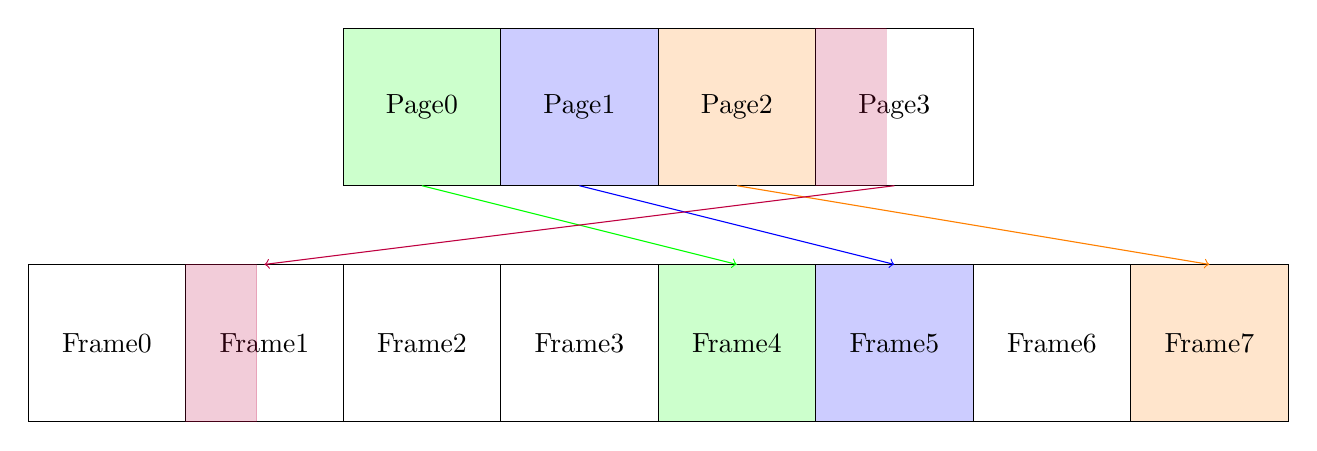
\begin{tikzpicture}
        \draw (-3, 0) node(p0)[rectangle, black, draw, minimum height = 2cm, minimum width = 2 cm, fill=green!20]{Page0};
        \draw (-1, 0) node(p1)[rectangle, black, draw, minimum height = 2cm, minimum width = 2 cm, fill=blue!20]{Page1};
        \draw (1, 0) node(p2)[rectangle, black, draw, minimum height = 2cm, minimum width = 2 cm, fill=orange!20]{Page2};
        \draw (3, 0) node(p3)[rectangle, black, draw, minimum height = 2cm, minimum width = 2 cm]{Page3};
        \filldraw[purple, opacity=0.2] (2, -1) rectangle (2.9, 1);
    

        \draw (-7, -3) node[rectangle, black, draw, minimum height = 2cm, minimum width = 2 cm]{Frame0} node[above=1cm](f0){};
        \draw (-5, -3) node(f1)[rectangle, black, draw, minimum height = 2cm, minimum width = 2 cm]{Frame1};
        \filldraw[purple, opacity=0.2] (-6, -4) rectangle (-5.1, -2);
        \draw (-3, -3) node(f2)[rectangle, black, draw, minimum height = 2cm, minimum width = 2 cm]{Frame2};
        \draw (-1, -3) node(f3)[rectangle, black, draw, minimum height = 2cm, minimum width = 2 cm]{Frame3};
        \draw (1, -3) node(f4)[rectangle, black, draw, minimum height = 2cm, minimum width = 2 cm, fill=green!20]{Frame4};
        \draw (3, -3) node(f5)[rectangle, black, draw, minimum height = 2cm, minimum width = 2 cm, fill=blue!20]{Frame5};
        \draw (5, -3) node(f6)[rectangle, black, draw, minimum height = 2cm, minimum width = 2 cm]{Frame6};
        \draw (7, -3) node(f7)[rectangle, black, draw, minimum height = 2cm, minimum width = 2 cm, fill=orange!20]{Frame7};
    
        \draw[green, ->] (-3, -1) -- (1, -2); 
        \draw[blue, ->] (-1, -1) -- (3, -2); 
        \draw[orange, ->] (1, -1) -- (7, -2); 
        \draw[purple, ->] (3, -1) -- (-5, -2); 
    \end{tikzpicture}\]
    Получаем таблицу страниц (находится в PCB у каждого процесса):
    \[\begin{tabular}{|c|c|c|c|c|}
        \hline
        Страница &0 & 1 & 2 & 3\\
        \hline
        Кадр & 4 & 5 & 7 & 1\\
        \hline
    \end{tabular}\]
    \begin{center}
        Кусочно-непрерываное отображение
    \end{center}
    Процессор -> логический адрес (Npage, offset) -> таблица страниц -> физический адрес (Nframe, offset) -> Память\\
    MMU (БУП) - memory management unit (блок управления памятью) 
    \begin{center}
        \bf Сегментно-страничная организация
    \end{center}
    Теперь логический адрес двумерный:\\
    (Nseg, soffset), где soffset = Npage$\cdot$size + poffset. Задаётся кортежем (Nseg, Npage, poffset).\\
    Физический адрес линейный $ = $ Nframe$\cdot$size + offset. Задаётся парой (Nframe, offset).\\
    Процессор -> (Nseg, soffset) -> ... -> (Nframe, offset)\\
    В ... входят:
    \begin{enumerate}
        \item Таблица сегментов
        \[\begin{tabular}{|c|c|}
            \hline
            Адрес & Размер\\
            \hline
             & \\
             \hline
             & \\
             \hline
             & \\
             \hline
        \end{tabular}\]
        Проверяем, что soffset не больше размера сегмента, иначе кидает segmentation fault. Если всё хорошо, получаем пару (Npage, poffset).
        \item Таблица страниц
        \[\begin{tabular}{|c|c|}
            \hline
            Страница & Кадр\\
            \hline
             & \\
             \hline
             & \\
             \hline
             & \\
             \hline
        \end{tabular}\]
        Из неё получаем искомую пару (Nframe, offset).
    \end{enumerate}
    \begin{center}
        \bf Многоуровневая таблица страниц
    \end{center}
    Таблица страниц процесса располагается в физическом адресном пространстве. При больших размерах таблицы страниц её размещение в последовательных кадрах памяти проблематично.\\
    Решение: разбить таблицу страниц на страницы, сделать таблицу страниц для таблицы страниц и поместить страницы в память в любом порядке (повторять, пока не залезет в память).\\
    При двухуровневой организации таблицы страниц логический адрес процесса описывается тройкой ($p_1$, $p_2$, d), где $p_1$ --- номер страницы в таблице страниц процесса, $p_2$ --- смещение внутри страницы $p_1$
    \begin{center}
        \bf Хэшированная таблица страниц
    \end{center}
    Номер страницы хэшируется, из хэш таблицы получаем номер кадра и переходим к физической памяти.
    \begin{center}
        \bf Ассоциативная память (TLB)
    \end{center}
    (page, offset) -> TLB -> (frame, offset)
    TLB (translation lookaside buffer):
    \[\begin{tabular}{|c|c|}
        \hline
        страница & кадр\\
        \hline
        &\\
        \hline
        &\\
        \hline
        &\\
        \hline
    \end{tabular}\]
    Если запись с нужной страницей есть, то мы её быстро получаем. Если нет, то нужно залезать в таблицу страниц.
    \subsection*{Расчёт среднего времени доступа}
    Обозначения:\\
    $t_0$ --- среднее время доступа к оперативной памяти. Пусть 100 наносекунд\\
    $t_1$ --- среднее время доступа к TLB. Пусть 10 наносекунд\\
    $h$ --- вероятность наличия информации в TLB (hit ratio). Пусть это 0.8.\\
    Среднее время доступа к данным при двухуровневой страничной схеме --- это:
    \[T = t_1 + ht_0 + (1 - h)\cdot 3t_0 = 10 + 80 + 60 = 150\]
    Без TLB:
    \[T = 3t_0 = 300\]
    В среднем требуется в два раза меньше времени.
    \begin{center}
        \bf Концепция виртуальной памяти
    \end{center}
    \begin{enumerate}
        \item Логическое адресное пространство процесса разбито на участки и линейно кусочно-непрерывно отображается. Недописал
        \item Недописал
        \item В оперативной физической памяти одновременно размещаются не все участки логического адресного пространства, а только их часть, остальные находятся во вторичной памяти.
        \item При обращении к участку логического адресного пространства, находящемуся во вторичной памяти, он подкачивается в оперативную память, возможно, с выталкиванием из нее некоторых неиспользующихся в данный момент участков.
    \end{enumerate}
    \begin{center}
        \bf Преимущества виртуальной памяти
    \end{center}
    \begin{enumerate}
        \item Процесс не ограничен объемом физической памяти. Упрощается разработка программ.
        \item Повышается степень мультипрограммирования.
        \item Выгрузка во вторичную память части процесса происходит быстрее, чем выгрузка всего процесса. Повышается эффективность работы системы, испольщующей среднесрочное планирование.
    \end{enumerate}
    \begin{center}
        \bf Изменения в таблице страниц.
    \end{center}
    Добавляем два бита к номеру страницы. Один из них отвечает за наличие страницы, второй (необязательный) --- бит модификации страница.\\
    При обращении к странице с нулевым битом наличия происходит исключительная ситуация page fault:
    \begin{enumerate}
        \item Выполнение команды прекращается --- hardware.
        \item Сохраняется часть контекста перед выполнением команды. Управление передается по заранее определенному адресу --- hardware
        \item Сохраняется оставшийся контекст --- hardware
        \item Страница подкачивается в память, возможно, с выталкиванием из памяти другой страницы --- software + hardware.
        \item Восстановление контекста. Повторное выполнение команды --- software + hardware.
    \end{enumerate}
    Бит модификации нужен для того, чтобы не закачивать немодифицированную страницу памяти на диск при необходимости её выкидывания из оперативной памяти (страница и так уже лежит на диске в неизменённом виде, то есть сохраняем только изменённые страницы).
    \begin{center}
        \bf Стратегии управления
    \end{center}
    \begin{enumerate}
        \item Стратегия выборки --- когда подкачивать страницу?
        \begin{itemize}
            \item По запросу (page fault $\Rightarrow$ подгрузили).
            \item С упреждением (по запросу + подгружаем соседние страницы)
        \end{itemize}
        \item Стратегия размещения --- куда подкачивать страницу?
        \item Стратегия замещения --- что из оперативной памяти убрать?
    \end{enumerate}
    \begin{center}
        \bf Алгоритмы замещения страниц
    \end{center}
    \subsection*{Виды алгоритмов}
    \begin{itemize}
        \item Локальные: процессу выделяется определённое количество кадров памяти, и только в этих кадрах он работает.
        \item Глобальные: при работе процесса можно использовать кадры других процессов.
    \end{itemize}
    Для анализа работы алгоритмов используется строка обращений процесса к памяти (строка запросов).\\
    Для локальных алгоритмво обычно используются сокращённые строки обращений. Если к некоторой странице обращаются несколько раз подряд, то записывается только первое такое обращение.
    \begin{center}
        \bf Локальные алгоритмы замещения
    \end{center}
    \subsection*{FIFO}
    \begin{center}
        \bf Аномалия Belady
    \end{center}
    Для некоторых строк запросов работа алгортима при увеличении количества выделенных кадров приводит к увеличению числа страничных нарушений.
    \subsection*{Определение}
    \underline{Стековые алгоритмы} --- алгоритмы, для которых при одной и той же строке запросов в один и тот же момент её обработки набор страниц в памяти для $n$ кадров всегд есть подмножество набора стрнаиц в памяти для $n + 1$ кадра, называются стековыми алгоритмами.\\
    Стековые алгоритмы не проявляют аномалии Belady.
\end{document}